%Motivation
\begin{figure*}
	\begin{center}
	  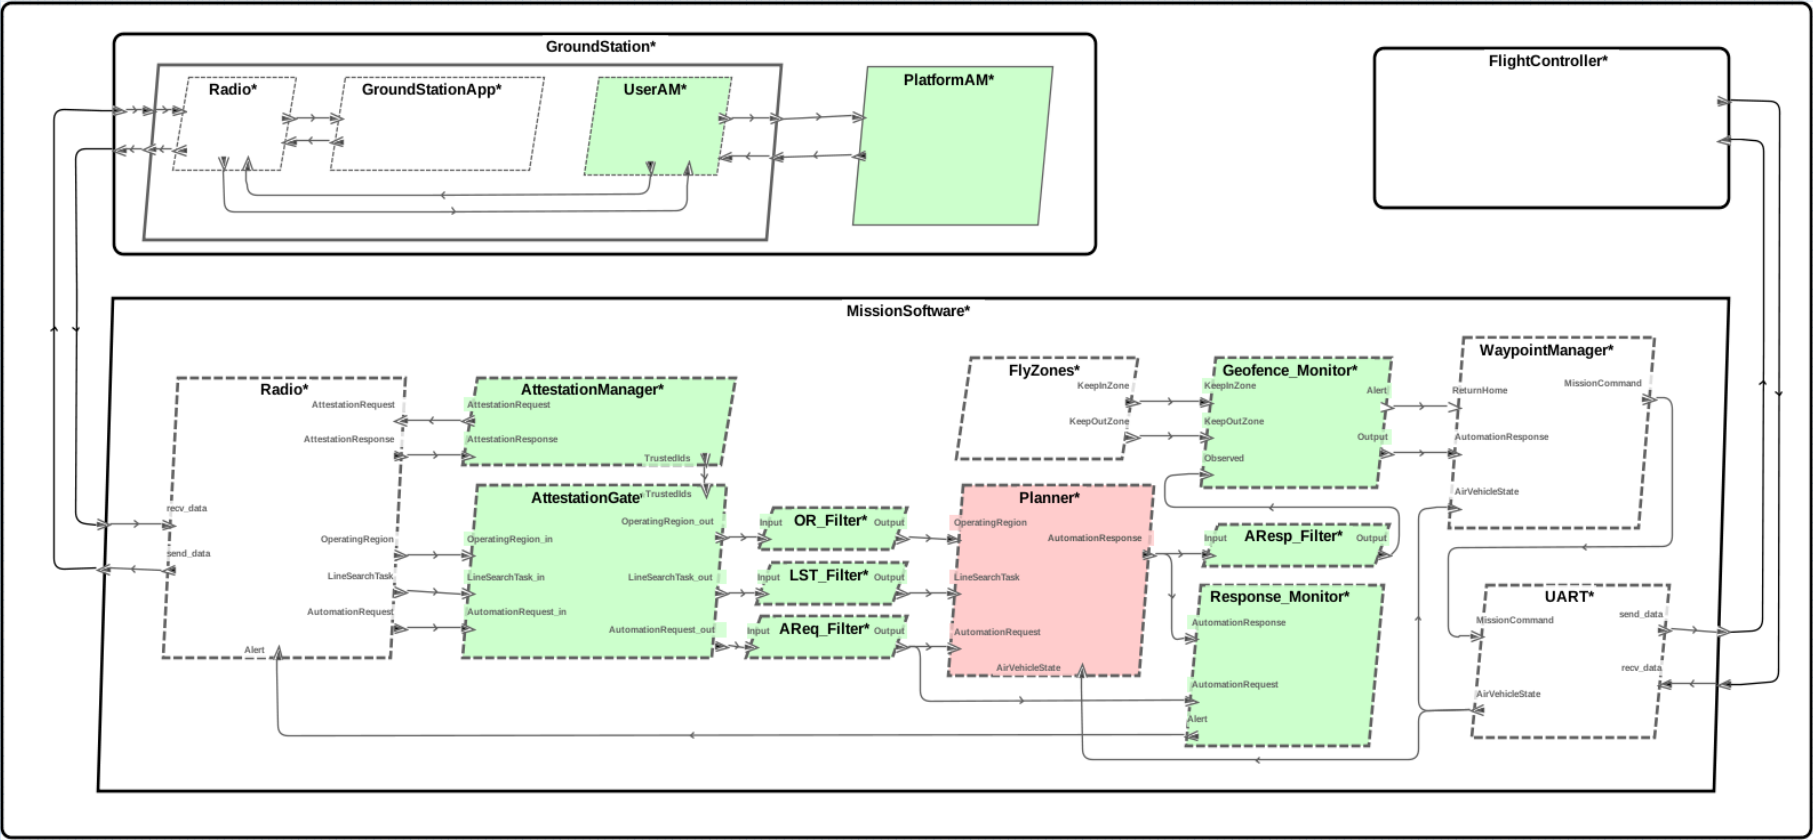
\includegraphics[width=\textwidth]{./figs/sw-hardened.png}
  \end{center}
	\caption{Cyber-resilient software architecture for UAV surveillance system. MAKE NAMES BIGGER, ADD GS AND FC} 
	\label{fig:sw-hardened} 
\end{figure*}

The example in \figref{fig:sw-hardened} shows an AADL model
% is a model-based design in the AADL OSATE tool 
of an unmanned air vehicle (UAV) for surveillance that was built with our \briefcase \ tools.  
We will use this example to explain how the tools work together to implement the system
and ensure its cyber-resiliency.  

The system includes a ground station computer and the aircraft, consisting of a mission computer and 
a flight control computer.  
The baseline (unhardened) mission computer included the four software components marked with asterisks: 
the radio for communication with the ground station (\emph{Radio}), 
the mission planning service (\emph{Planner}, provided as legacy software running on Linux), 
flight plan waypoint segmentation (\emph{WaypointManager}), 
and a serial interface to communicate with the flight control computer (\emph{UART}).

%\briefcase\ integrates four key formal methods in the model-based engineering workflow:
%verification via the Assume Guarantee REasoning Environment (\agree);
%synthesis of high-assurance components by means of the Semantic
%Properties of Language and Automata Theory tool (\splat); synthesis
%of inter-component communication by the High Assurance Modeling and
%Rapid engineering for embedded systems tool (\hamr); and the \selFour\ verified microkernel.
%Each component in the unhardened system, and the interface for the top-level software component, is
%formally specified with an AGREE contract stating assumptions on inputs and guarantees on outputs
%under the assumptions.
%\agree\ proves the unhardened implementation obeys the composition of these contracts. 
%
Cyber-threat analysis tools are used to analyze to original functional model of the system, 
identifying the ground station and the mission planning
service as primary sources of cyber attacks.
Seven new cyber requirements are added to the unhardened system that require ground station
trust assessment, message integrity checks, and run-time monitoring of several conditions.
The existing behavioral contracts in the unhardened system are strengthened to reflect these new requirements.
%\agree\ proves the unhardened system under these contracts fails verification. 

Design engineers use \briefcase\ to transform the baseline system model to that shown in
\figref{fig:sw-hardened}.  Automated model transformations address the cyber requirements by inserting  
new high-assurance components (shown in green) and targeting the seL4 kernel to enforce separation between components.
The \emph{AttestationManager} establishes the identity of trusted ground stations while
the \emph{AttestationGate} only passes messages from trusted sources.  The three 
filters  (\emph{OR\_Filter}, \emph{LST\_Filter}, \emph{AReg\_Filter}, and \emph{AResl\_Filter}) 
only pass well-formed messages received from the Radio. A filter on the output of the Planner ensures 
that only well-formed flight plans are sent to the WaypointManager.  
Two run-time monitors alert the system to suspicious behaviors from the Planner such as flight plans that enter keep-out zones or leave
keep-in zones (\emph{Geofence\_Monitor}) or unrequested mission plans (\emph{Response\_Monitor}).
The interface behavior of these high-assurance components, with the exception of attestation, is
specified with assume-guarantee contracts (e.g., a filter makes no assumptions on input and only
passes inputs that are syntactically well-formed).
%\agree\ proves the hardened system ensures the added cyber requirements.

The model is further transformed to move the mission planning service into a 
Linux virtual machine hosted on the \selFour \ microkernel. This permits us to run the
legacy mission planner code without modification or porting and isolate any 
unintended behaviors.  
The target platform requires a static real-time schedule that is provided in the model.
A transformation on the assume-guarantee contracts incorporates that schedule into the model
for verification of the cyber requirements.

%\resolint\ certifies the hardened model is ready for synthesis.
%\splat\ synthesizes high-assurance components from their \agree\ contracts to the target platform.
%It includes proof certificates that the binaries have assumptions that are no stronger than those on
%the original contracts and guarantees that are no weaker than those on the original contracts (e.g.,
%safe substitution).
%\hamr\ synthesizes all the inter-component communication primitives from the AADL model.
%That synthesis includes a proof certificate that the resulting communication channels defined in
%\selFour\ are only those defined in the AADL model.
%
%\resolute\ builds an assurance case for the entire system.
%That assurance case includes evidences for every requirement including proof certificates from
%\agree, \splat, and \hamr.
